%% figures/fig3_pattern_cycle_grid.tex
%% Fig.3 — 2×3 work pattern × cycle ablation heatmap (단일 컬럼 fit)

\begin{figure}[t]
\centering
\resizebox{0.90\columnwidth}{!}{%
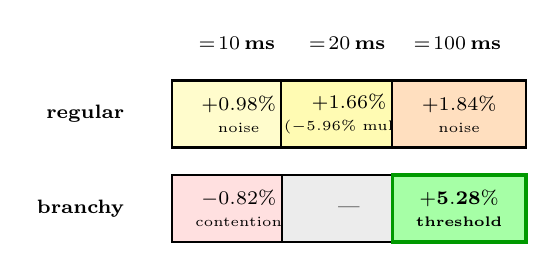
\begin{tikzpicture}[
    x=1.4cm, y=1.0cm,
    cell/.style={rectangle, draw, minimum width=1.7cm, minimum height=0.85cm,
                 align=center, font=\scriptsize, thick, inner sep=1pt},
    header/.style={font=\scriptsize\bfseries, align=center},
    rowlabel/.style={font=\scriptsize\bfseries, align=center, anchor=east},
]
% Column headers
\node[header] at (0, 1.5)  {$\tcpu\!=\!10$\,ms};
\node[header] at (1.0, 1.5) {$\tcpu\!=\!20$\,ms};
\node[header] at (2.0, 1.5) {$\tcpu\!=\!100$\,ms};

% Row labels
\node[rowlabel] at (-0.95, 0.6) {regular};
\node[rowlabel] at (-0.95, -0.6) {branchy};

% Regular row
\node[cell, fill=yellow!20] at (0, 0.6)
    {$+0.98\%$\\\tiny noise};
\node[cell, fill=yellow!30] at (1.0, 0.6)
    {$+1.66\%$\\\tiny ($-5.96\%$ multi)};
\node[cell, fill=orange!25] at (2.0, 0.6)
    {$+1.84\%$\\\tiny noise};

% Branchy row
\node[cell, fill=red!12] at (0, -0.6)
    {$-0.82\%$\\\tiny contention};
\node[cell, fill=gray!15] at (1.0, -0.6) {---};
\node[cell, fill=green!35, very thick, draw=green!60!black] at (2.0, -0.6)
    {$\mathbf{+5.28\%}$\\\tiny\textbf{threshold}};
\end{tikzpicture}%
}
\caption{작업 패턴 $\times$ 주기 2$\times$3 ablation. branchy $\times$ 100\,ms 만 유의 임계점 $+5\,\%$ 도달. 박자 정렬 (Theorem~\ref{thm:alignment}) 과 prefetcher 억제의 결합 효과 (\S\ref{sec:mechanism}).}
\label{fig:pattern-cycle-grid}
\end{figure}
